\chapter{Workflows in \mutation}
\label{ch:workflows}

\newthought{\mutation\ workflows} consist of components that read, process, and visualize data. We refer to these components as ``widgets'' We place the widgets on a drawing board called the ``canvas'' to design a workflow. Widgets communicate by sending information along their communication channel. Output from one widget can be used as input to another.

\begin{figure*}[h]
  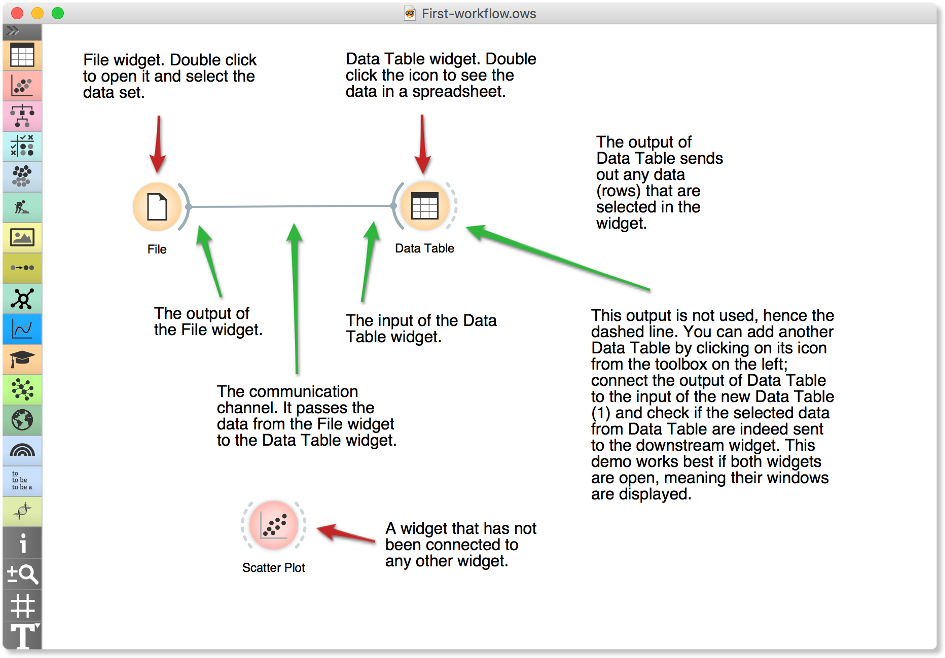
\includegraphics[width=\linewidth]{workflow-fig1.png}%
  \caption{\textbf{\textsf{A simple workflow with two connected widgets and one widget without connections. The outputs of a widget appear on the right, while the inputs appear on the left.}}}
  \label{fig:workflow-fig1}
\end{figure*}

We construct workflows by dragging widgets onto the canvas and connecting them by drawing a line from the transmitting widget to the receiving widget. The widget's outputs are on the right, and the inputs on the left. In the workflow above, the \widget{File} widget sends data to the \widget{Data Table} widget.
\newpage
Start by constructing a workflow that consists of a File widget, two \widget{Scatter Plot} widgets and two Data Table widgets:

\begin{figure}[h]
  \centering
  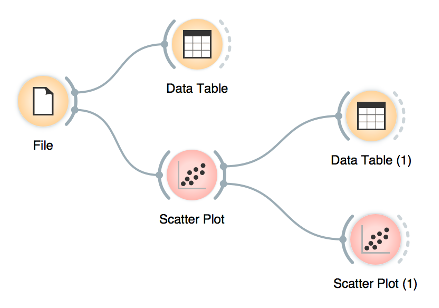
\includegraphics[width=80mm]{workflow-fig2.png}%
  \caption{\textbf{\textsf{A workflow with a File widget that reads the data from a disk and sends it to the Scatter Plot and Data Table widget. The Data Table renders the data in a spreadsheet, while the Scatter Plot visualizes it. The plot's selected data points are sent to two other widgets: Data Table (1) and Scatter Plot (1).}}}
  \label{fig:workflow-fig2}
\end{figure}

The \widget{File} widget reads data from your local disk. Open the \widget{File} widget by double-clicking its icon. \mutation\ comes with several pre-loaded data sets. From these (``Browse documentation data sets...''), choose \textit{brown-selected.tab}, a yeast gene expression data set.

\begin{figure}[h]
  \centering
  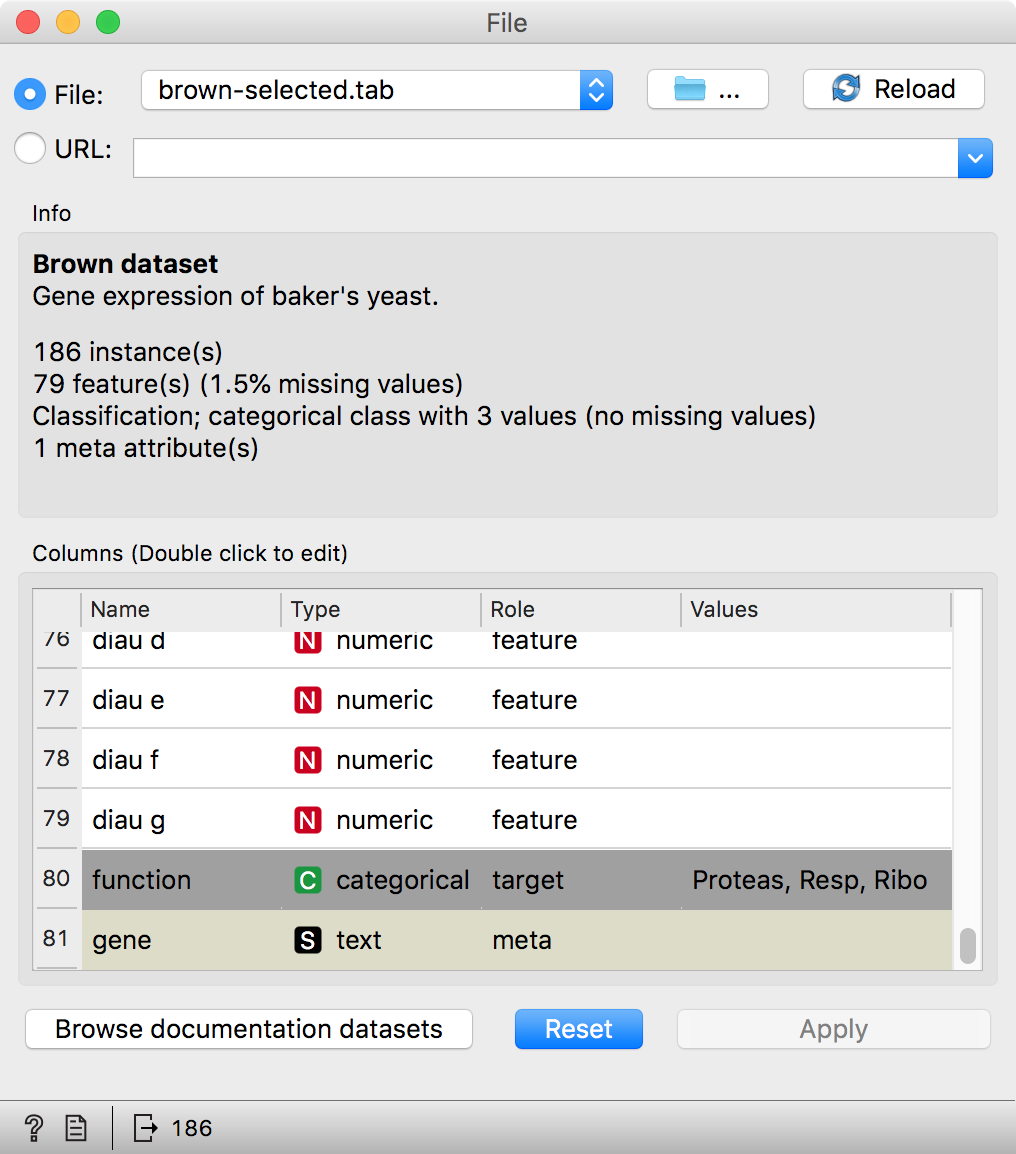
\includegraphics[width=0.9\linewidth]{file-brown.png}%
  \caption{\textbf{\textsf{\mutation\ workflows often start with a File widget. The brown-selected data set comprises 186 rows (genes) and 81 columns. Out of the 81 columns, 79 contain gene expressions of baker's yeast under various conditions, one column (marked as a "meta attribute") provides gene names, and one column contains the "class" value or gene function.}}}
  \label{fig:workflow-fig3}
\end{figure}

After you load the data:
\begin{enumerate}
\item Open the other widgets.
\item Select a few data points in the \widget{Scatter Plot} widget and watch as they appear in the \widget{Data Table (1)}.
\item Use a combination of two \widget{Scatter Plot} widgets, where the second scatter plot shows a detail from a smaller region selected in the first scatter plot.
\end{enumerate}

The following is a side note, but it won't hurt. The scatter plot for a pair of random features does not provide much information on gene function. Does this change with a different choice of feature pairs in the visualization? \textit{Rank projections} at the button on the top left of the Scatter Plot widget can help you find a good feature pair. How do you think this works? Could the suggested pairs of features be helpful to a biologist?

\begin{marginfigure}[4cm]
  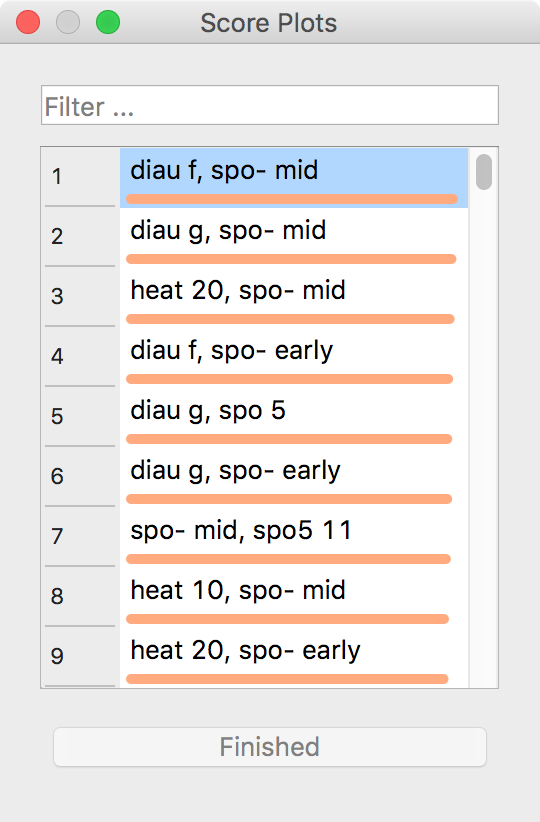
\includegraphics[width=0.9\linewidth]{score-plots.png}
  \caption{\textbf{\textsf{Scatter Plot and Ranking}}}
\end{marginfigure}

\begin{figure}
  \centering
  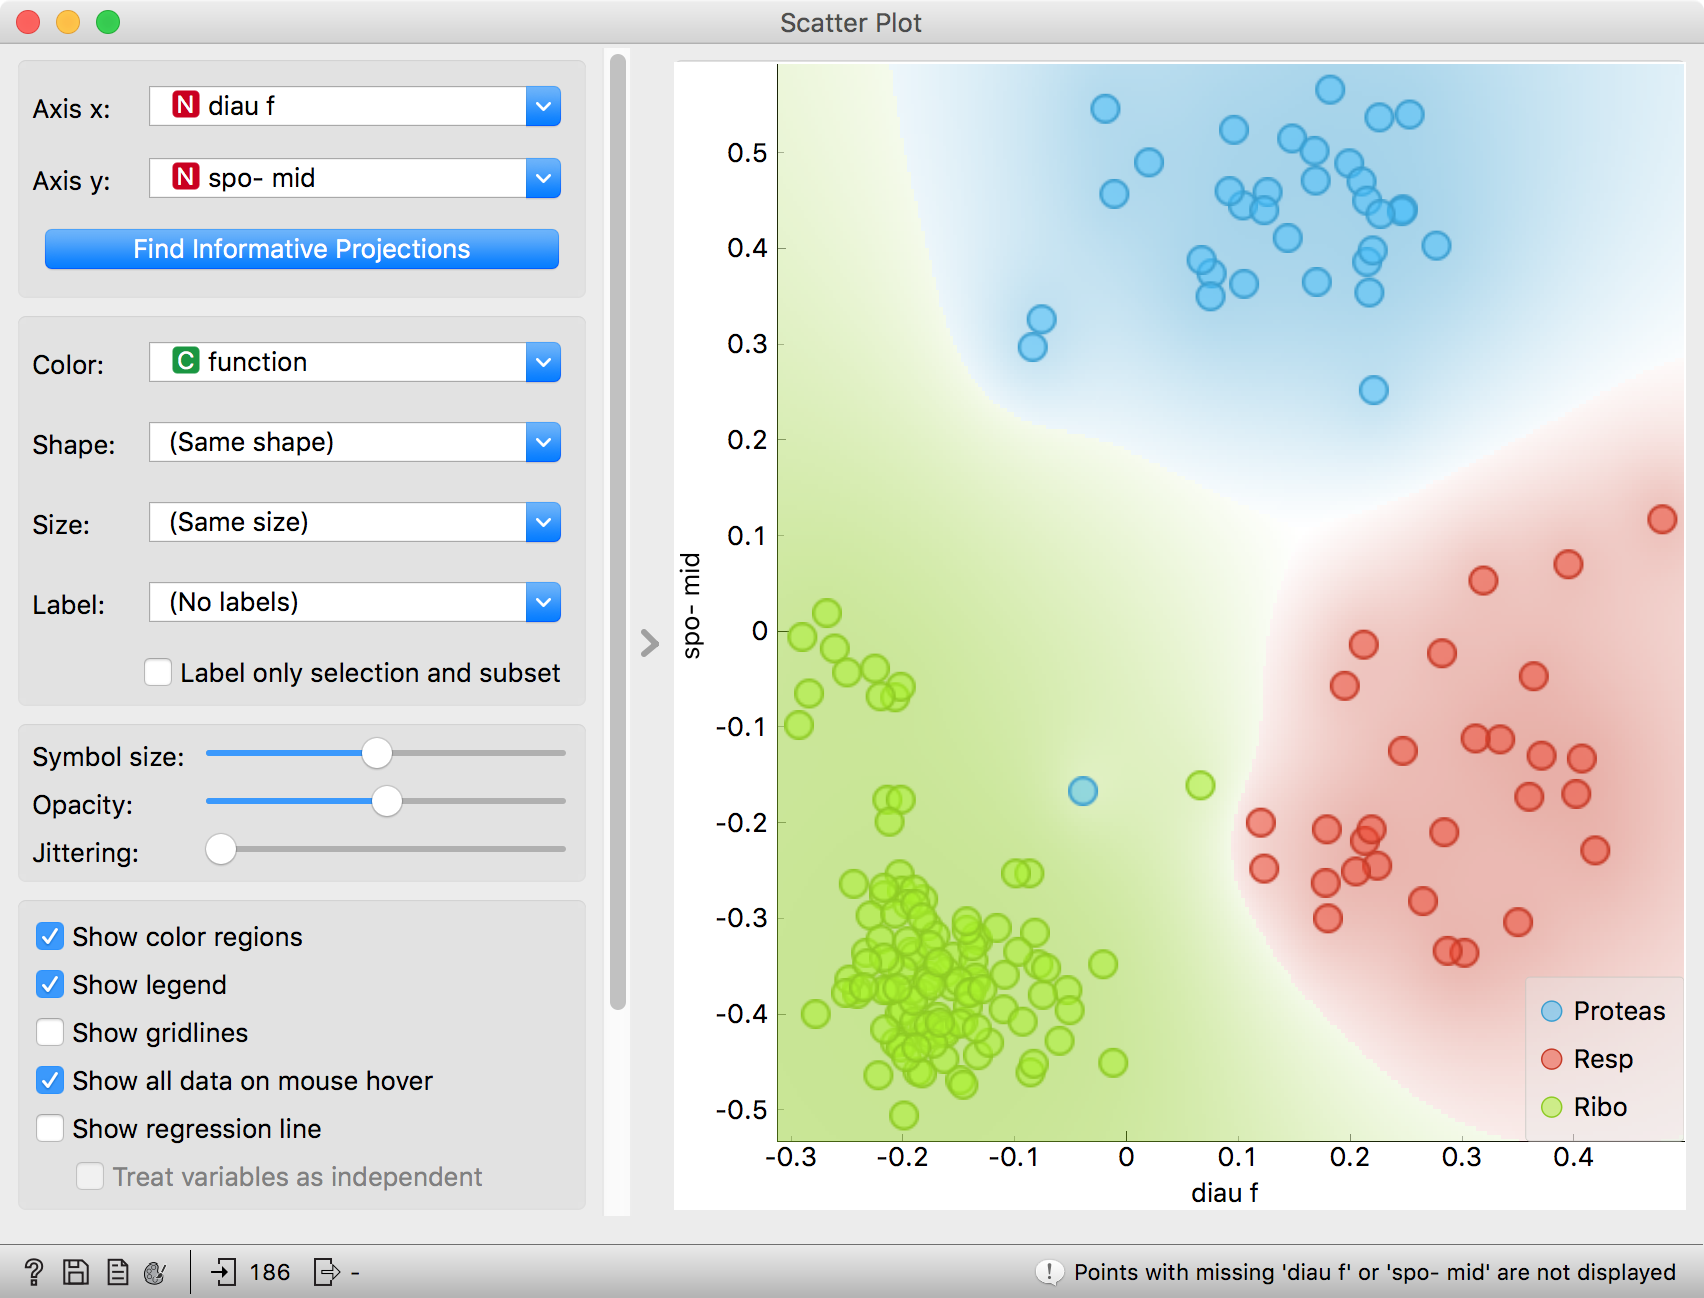
\includegraphics[width=\linewidth]{scatterplot-brown.png}
  \label{fig:workflow-scatterplot}
\end{figure}

We can connect the output of the \widget{Data Table} widget to the \widget{Scatter Plot} widget to highlight the chosen data instances (rows) in the scatter plot.

\begin{figure}
%   \centering
  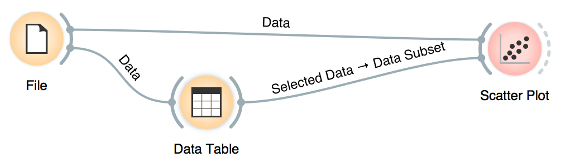
\includegraphics[width=100mm]{workflow-fig5.png}
  \caption{\textbf{\textsf{In this workflow, we have switched on the option "Show channel names between widgets" in File/Preferences.}}}
  \label{fig:workflow-fig5}
\end{figure}

How does \mutation\ distinguish between the primary data source and the data selection? It uses the first connected signal as the entire data set and the second one as its subset. To make changes or to check what is happening under the hood, double click on the line connecting the two widgets.
\newpage

\begin{figure*}[h]
%   \centering
  \flushright
  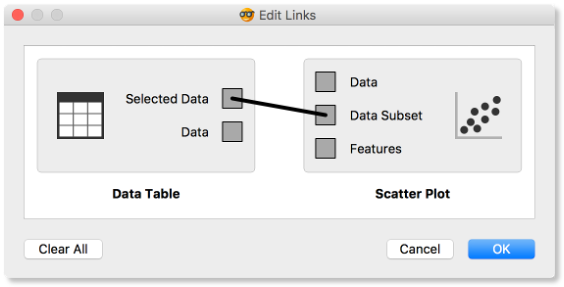
\includegraphics[width=100mm]{workflow-fig6.png}
\label{fig:workflow-fig6}%
\end{figure*}

The rows in the data set we are exploring in this lesson are gene profiles. We could perhaps use widgets from the Bioinformatics add-on to get more information on the genes we selected in any of the \mutation\ widgets.

\marginnote{\textbf{\textsf{\mutation\ comes with a basic set of widgets for data input, preprocessing, visualization and modeling. For other tasks, like text mining, network analysis, and bioinformatics, there are add-ons. Check them out by selecting Add-ons... from the Options menu.}}}

\begin{figure*}[h]
%   \centering
  \flushright
  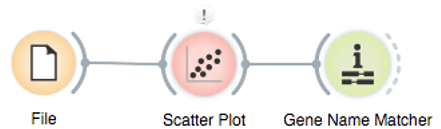
\includegraphics[width=80mm]{workflow-fig7.png}%
\label{fig:workflow-fig7}%
\end{figure*}
